
\Scene{2}[Another part of the island.]

\begin{figure}[t!]
\centering
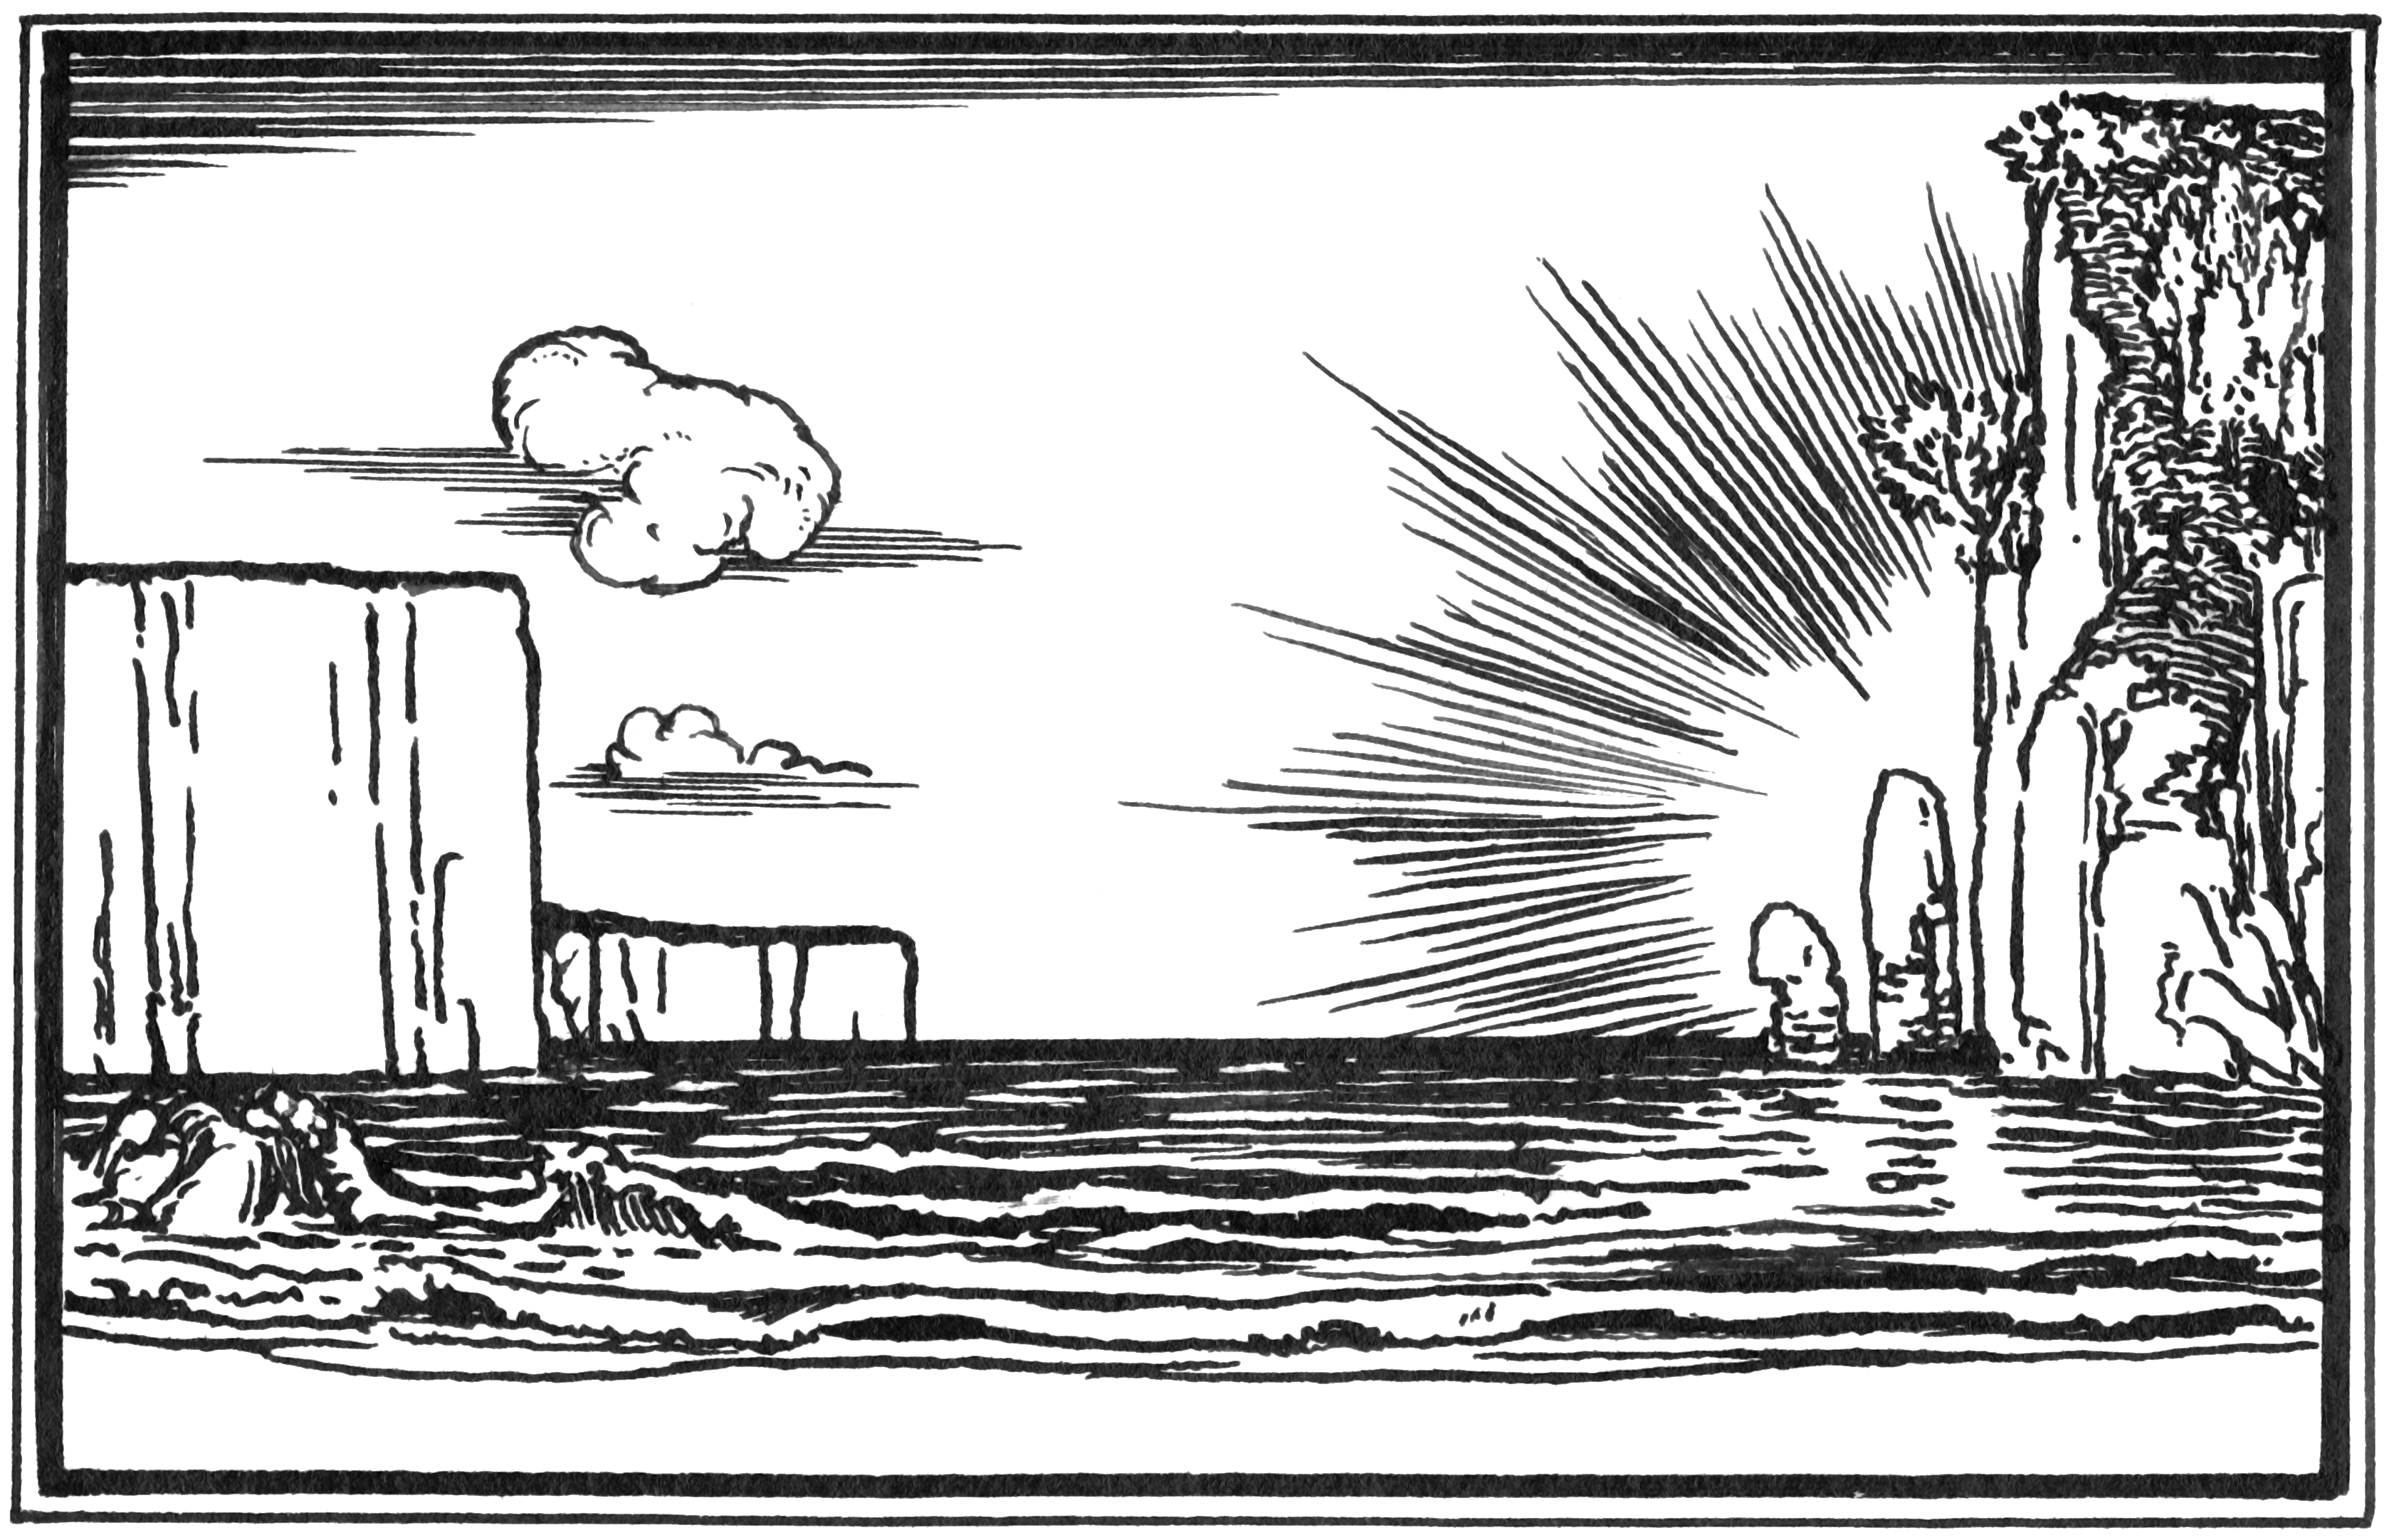
\includegraphics[width=\headerwidth]{3iiheadpiece}
\end{figure}
   
\enter{\textsc{Caliban}, \textsc{Stephano}, and \textsc{Trinculo}}

\begin{letter} %dropcap
	\begin{tikzpicture}[remember picture, overlay]
		\node (dropcap) at ($(current page.west)+(2.5cm,-4cm)$) {
\includegraphics[width=0.125\linewidth]{3iidropcapT}};
	\end{tikzpicture}
\end{letter}

\begin{a4} %dropcap
	\begin{tikzpicture}[remember picture, overlay]
		\node (dropcap) at ($(current page.west)+(2.5cm,-2.2cm)$) {
\includegraphics[width=0.115\linewidth]{3iidropcapT}};
	\end{tikzpicture}
\end{a4}
	
\verseline[Stephano]{\hspace{1.5em}ell not me; when the butt is out, we will drink water; not a drop before: therefore bear up, and board 'em. Servant-monster, drink to me.}

\verseline[Trinculo]{Servant-monster! the folly of this island! They say there's but five upon this isle: we are three of them; if th' other two be brained like us, the state totters.}

\verseline[Stephano]{Drink, servant-monster, when I bid thee: thy eyes are almost set in thy head.}

\verseline[Trinculo]{Where should they be set else? he were a brave monster indeed, if they were set in his tail.}

\verseline[Stephano]{My man-monster hath drown'd his tongue in sack: for my part, the sea cannot drown me; I swam, ere I could recover the shore, five and thirty leagues off and on. By this light, thou shalt be my lieutenant, monster, or my standard.}

\verseline[Trinculo]{Your lieutenant, if you list; he's no standard.}





\verseline[Stephano]{We'll not run, Monsieur Monster.}

\verseline[Trinculo]{Nor go neither; but you'll lie like dogs and yet say nothing neither.}

\verseline[Stephano]{Moon-calf, speak once in thy life, if thou beest a good moon-calf.}

\verseline[Caliban]{How does thy honour? Let me lick thy shoe. I'll not serve him; he's not valiant.}

\verseline[Trinculo]{Thou liest, most ignorant monster: I am in case to justle a constable. Why, thou deboshed fish thou, was there ever man a coward that hath drunk so much sack as I to-day? Wilt thou tell a monstrous lie, being but half a fish and half a monster?}

\verseline[Caliban]{Lo, how he mocks me! wilt thou let him, my lord?}

\verseline[Trinculo]{<Lord> quoth he! That a monster should be such a natural!}

\verseline[Caliban]{Lo, lo, again! bite him to death, I prithee.}

\verseline[Stephano] {Trinculo, keep a good tongue in your head: if you prove a mutineer,—the next tree! The poor monster's my subject and he shall not suffer indignity.}

\verseline[Caliban]{I thank my noble lord. Wilt thou be pleased to hearken once again to the suit I made to thee?}

\verseline[Stephano]{Marry, will I. kneel and repeat it; I will stand, and so shall Trinculo.}
	
\enter{\textsc{Ariel}, invisible}

\verseline[Caliban]{As I told thee before, I am subject to a tyrant, a sorcerer, that by his cunning hath cheated me of the island.}

\verseline[Ariel]{Thou liest.}

\verseline[Caliban]{Thou liest, thou jesting monkey, thou: I would my valiant master would destroy thee! I do not lie.}

\verseline[Stephano]{Trinculo, if you trouble him any more in's tale, by this hand, I will supplant some of your teeth.}

\verseline[Trinculo]{Why, I said nothing.}

\verseline[Stephano]{Mum, then, and no more. Proceed.}

\begin{verse_speech}[Caliban] 
I say, by sorcery he got this isle;\\
From me he got it. if thy greatness will\\
Revenge it on him,—for I know thou darest,\\
But this thing dare not,—
\end{verse_speech}

\verseline[Stephano]{That's most certain.}

\verseline[Caliban]{Thou shalt be lord of it and I'll serve thee.}

\begin{verse_speech}[Stephano] How now shall this be compassed?
Canst thou bring me to the party?
\end{verse_speech}

\begin{verse_speech}[Caliban] 
Yea, yea, my lord: I'll yield him thee asleep,\\
Where thou mayst knock a nail into his bead.
\end{verse_speech}


\verseline[Ariel]{Thou liest; thou canst not.}

\begin{verse_speech}[Caliban] 
What a pied ninny's this! Thou scurvy patch!\\
I do beseech thy greatness, give him blows\\
And take his bottle from him: when that's gone\\
He shall drink nought but brine; for I'll not show him
Where the quick freshes are.
\end{verse_speech}

\verseline[Stephano]{Trinculo, run into no further danger: interrupt the monster one word further, and, by this hand, I'll turn my mercy out o' doors and make a stock-fish of thee.}

\verseline[Trinculo]{Why, what did I? I did nothing. I'll go farther off.}

\verseline[Stephano]{Didst thou not say he lied?}

\verseline[Ariel]{Thou liest.}

\begin{verse_speech}[Stephano] 
Do I so? take thou that.
	
	\stage{Beats \textsc{Trinculo}}
	
As you like this, give me the lie another time.
\end{verse_speech}

\begin{letter}
	\begin{figure}[bt]
\centering
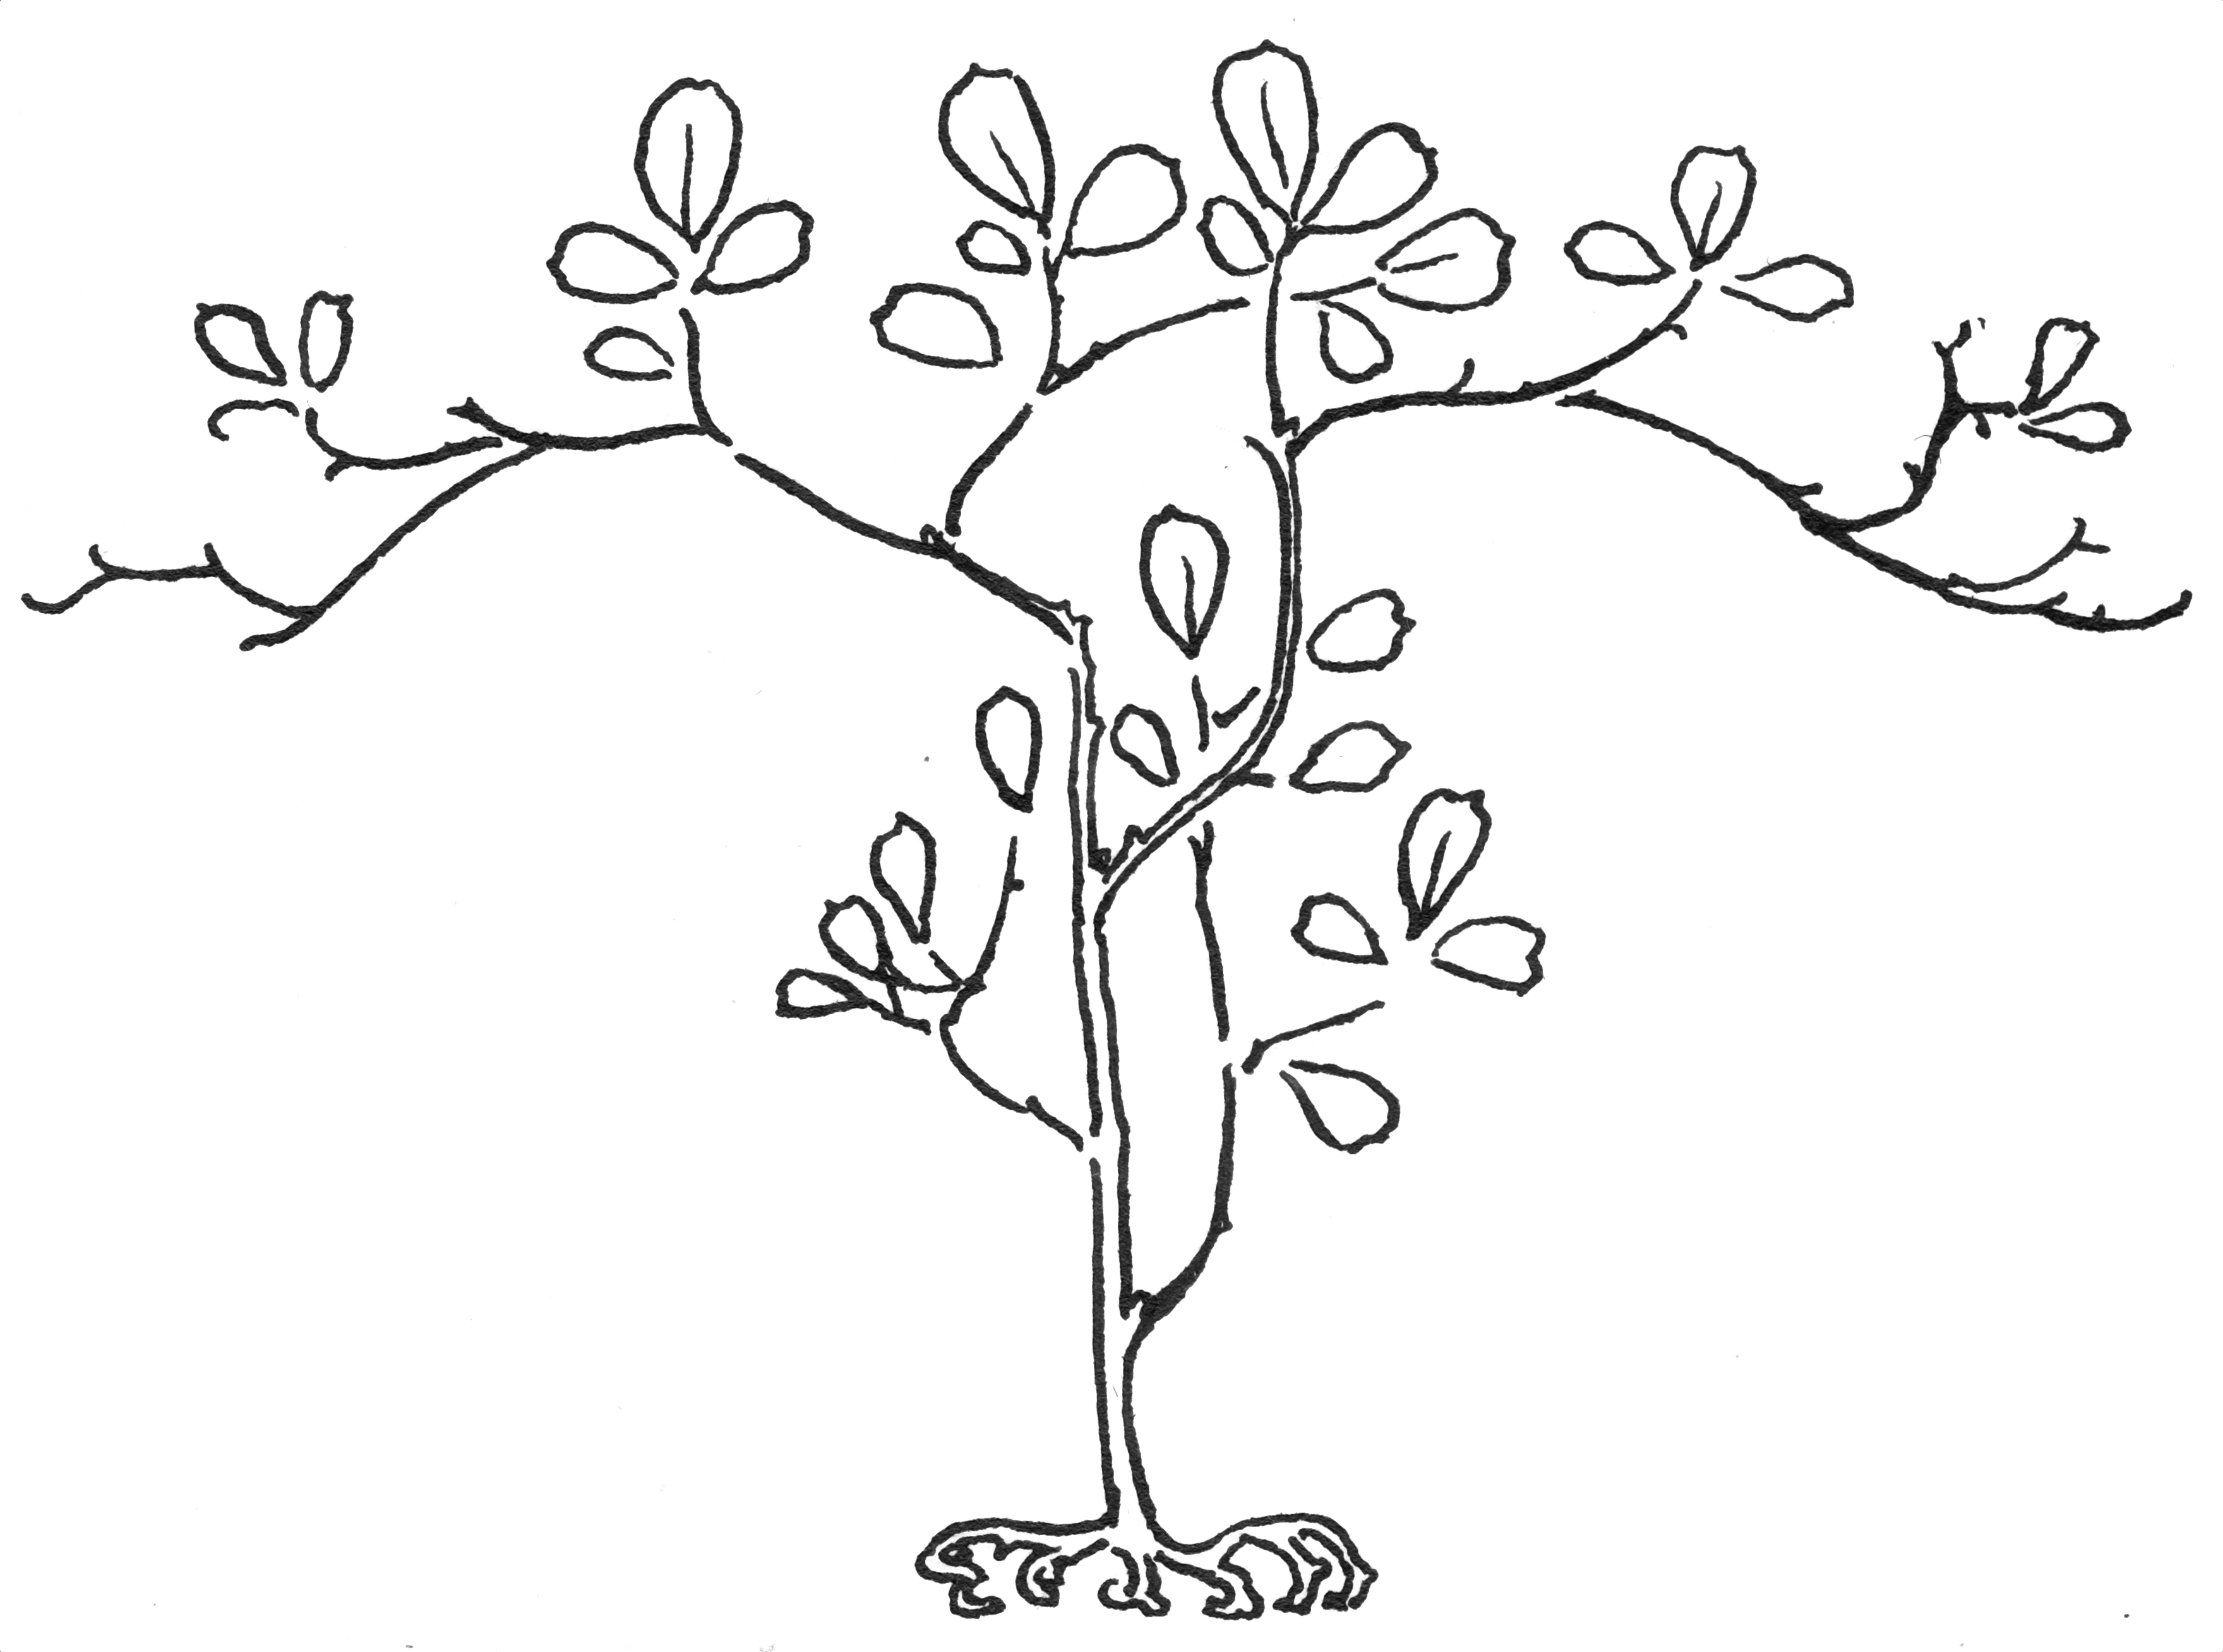
\includegraphics[width=.6\textwidth]{tree}
\end{figure}
% \begin{center}
% 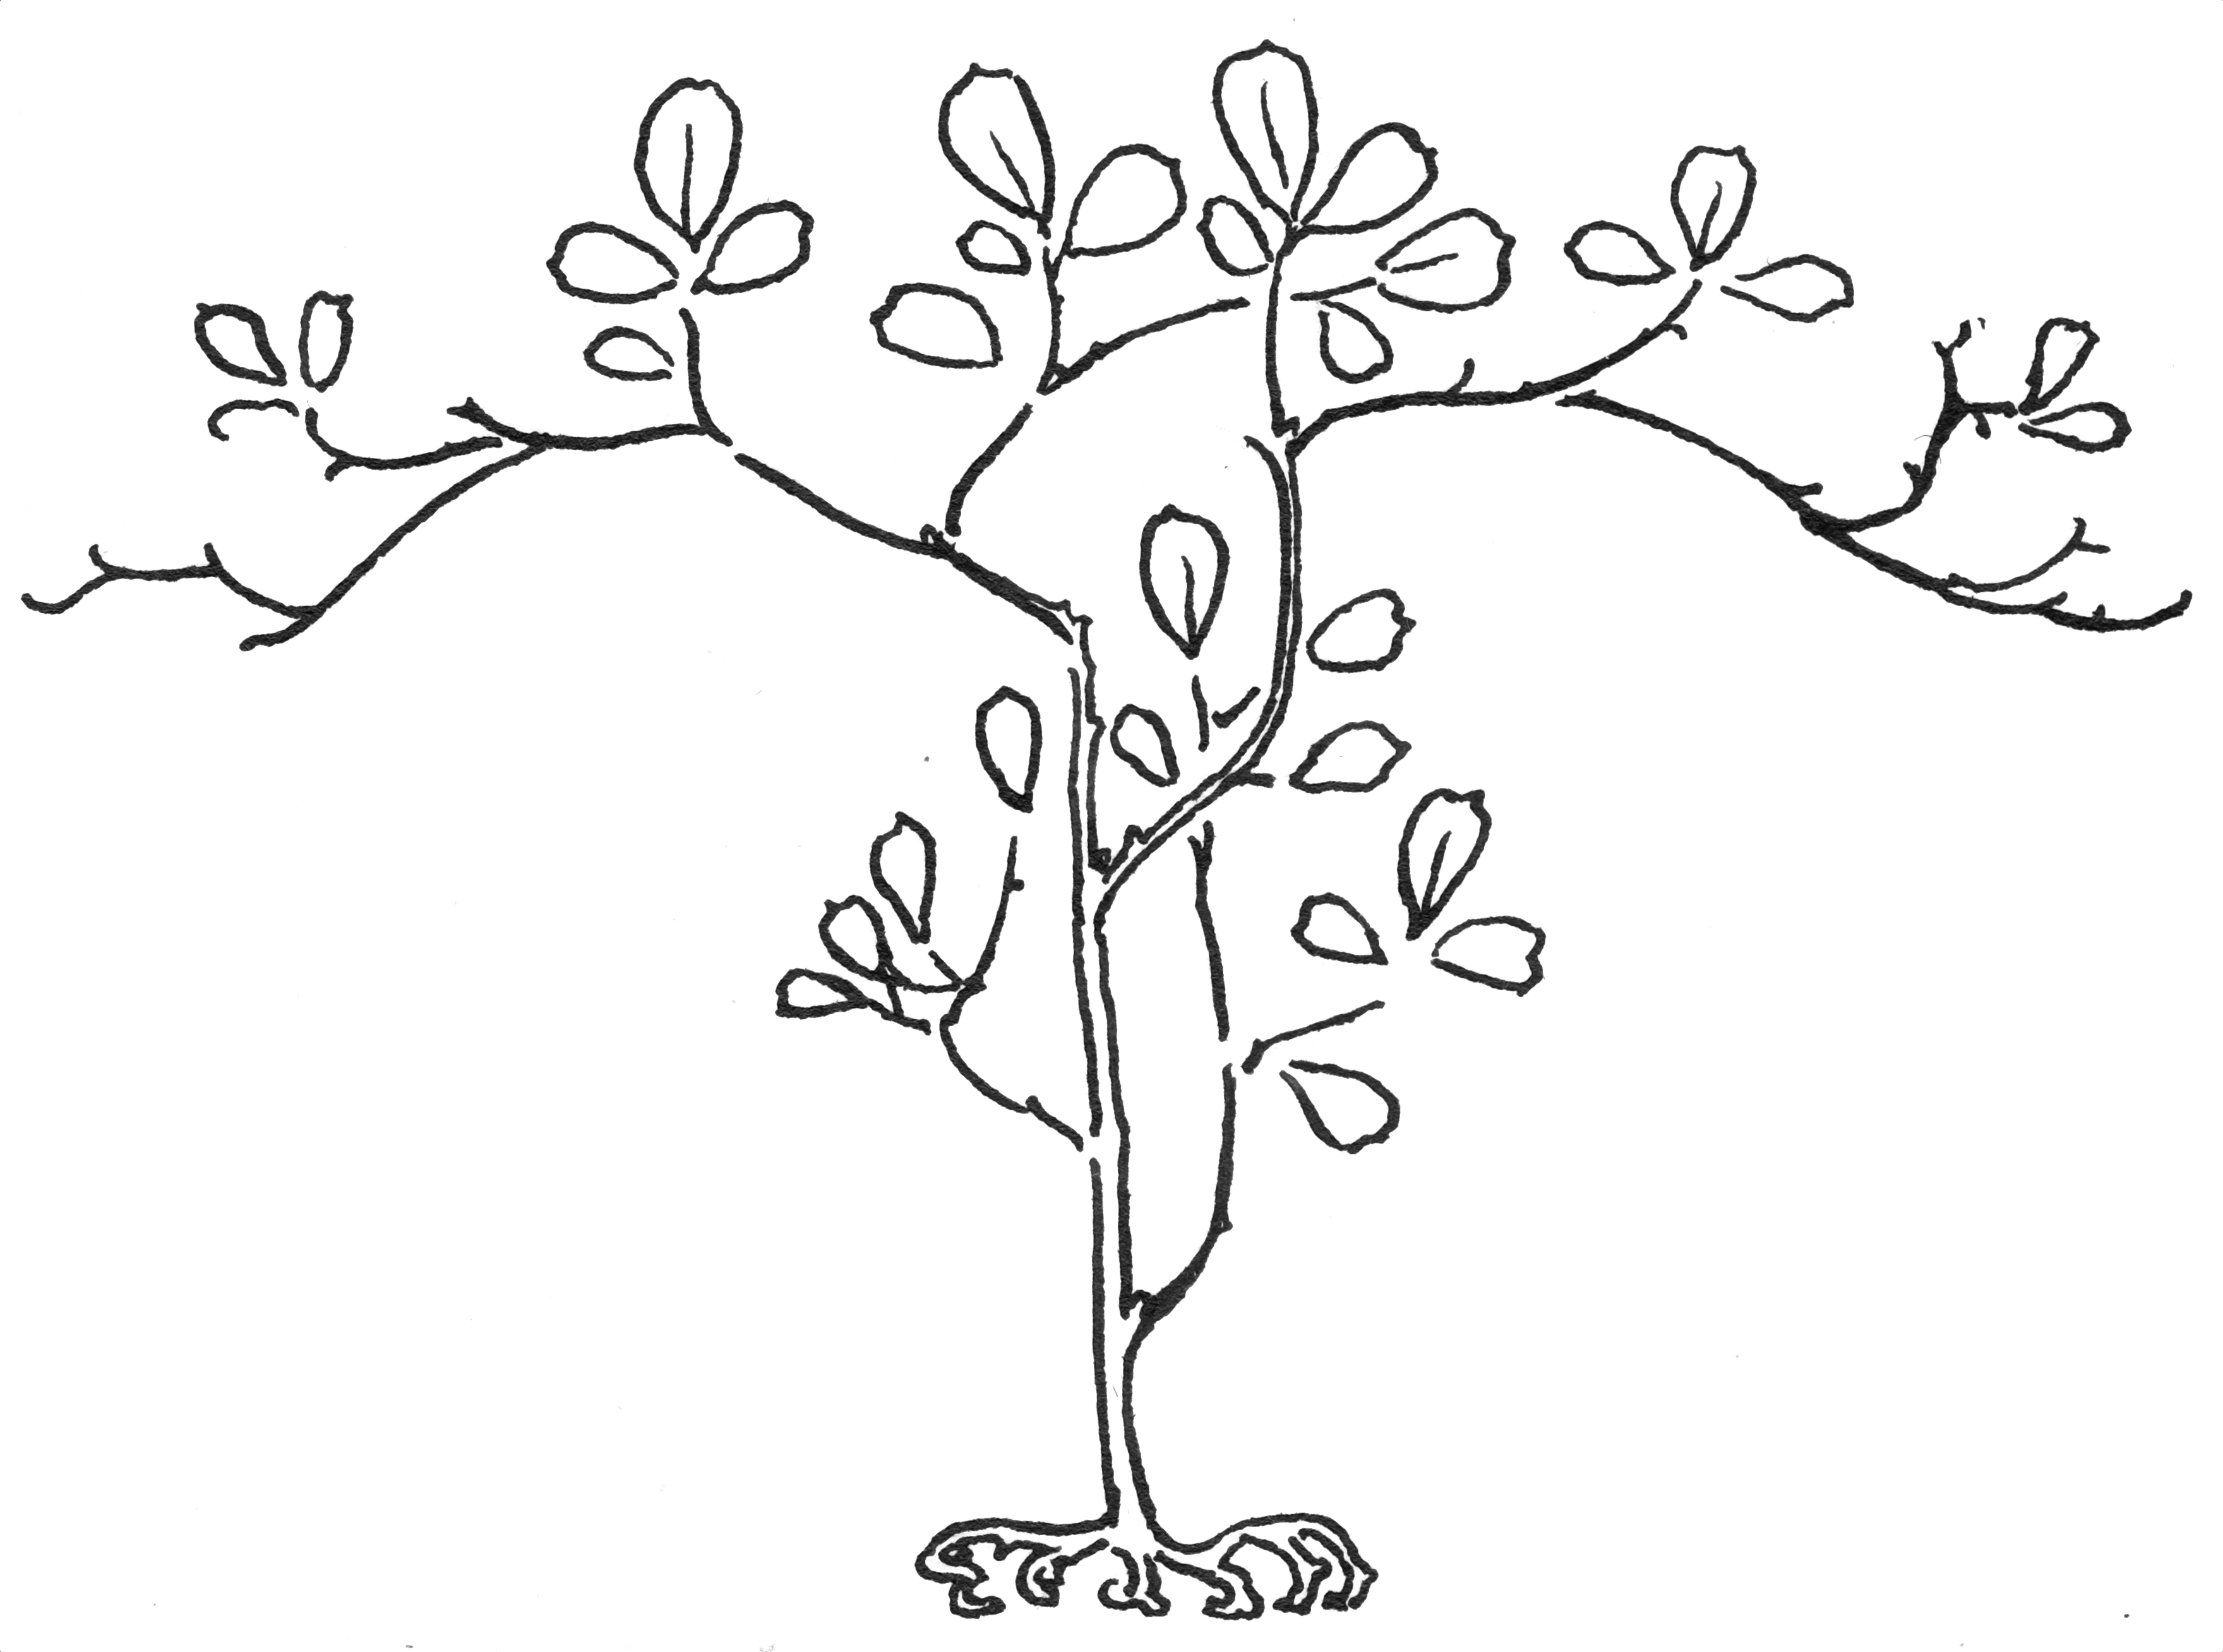
\includegraphics[width=]{tree}
% \end{center}
\end{letter}

\verseline[Trinculo]{I did not give the lie. Out o' your wits and bearing too? A pox o' your bottle! this can sack and drinking do. A murrain on your monster, and the devil take your fingers!}
	
\verseline[Caliban]{Ha, ha, ha!}

\verseline[Stephano]{Now, forward with your tale. Prithee, stand farther off.}

\begin{verse_speech}[Caliban]
Beat him enough: after a little time\\
I'll beat him too.
\end{verse_speech}

\begin{pictures}
	
\begin{bwbigpic}
	[\picwidth]
	{3iifight}
	{}
\end{bwbigpic}

\end{pictures}

\verseline[Stephano]{Stand farther. Come, proceed.}

\begin{verse_speech}[Caliban] 
Why, as I told thee, 'tis a custom with him,\\
I' th' afternoon to sleep: there thou mayst brain him,\\
Having first seized his books, or with a log\\
Batter his skull, or paunch him with a stake,\\
Or cut his wezand with thy knife. Remember\\
First to possess his books; for without them\\
He's but a sot, as I am, nor hath not\\
One spirit to command: they all do hate him\\
As rootedly as I. Burn but his books.\\
He has brave utensils,—for so he calls them—\\
Which when he has a house, he'll deck withal\\
And that most deeply to consider is\\
The beauty of his daughter; he himself\\
Calls her a nonpareil: I never saw a woman,\\
But only Sycorax my dam and she;\\
But she as far surpasseth Sycorax\\
As great'st does least.
\end{verse_speech}

\verseline[Stephano]{Is it so brave a lass?}

\begin{verse_speech}[Caliban] 
Ay, lord; she will become thy bed, I warrant.\\
And bring thee forth brave brood.
\end{verse_speech}

\verseline[Stephano] {Monster, I will kill this man: his daughter and I will be king and queen—save our graces!—and Trinculo and thyself shall be viceroys. Dost thou like the plot, Trinculo?}

\verseline[Trinculo]{Excellent.}

\verseline[Stephano]{Give me thy hand: I am sorry I beat thee; but, while thou livest, keep a good tongue in thy head.}

\begin{verse_speech}[Caliban] 
Within this half hour will he be asleep:
Wilt thou destroy him then?
\end{verse_speech}

\verseline[Stephano]{Ay, on mine honour.}

\verseline[Ariel]{This will I tell my master.}

\begin{verse_speech}[Caliban] 
Thou makest me merry; I am full of pleasure:\\
Let us be jocund: will you troll the catch\\
You taught me but while-ere?
\end{verse_speech}

\begin{verse_speech}[Stephano] At thy request, monster, I will do reason, any
reason. Come on, Trinculo, let us sing.
\stage{Sings}
\begin{song}
\songline{Flout 'em and scout 'em}
\songline{And scout 'em and flout 'em}
\songline{Thought is free.}
\end{song}
\end{verse_speech}

\verseline[Caliban]{That's not the tune.}
	
\stage{\textsc{Ariel} plays the tune on a tabour and pipe}

\verseline[Stephano]{What is this same?}

\verseline[Trinculo]{This is the tune of our catch, played by the picture of Nobody.}

\verseline[Stephano]{If thou beest a man, show thyself in thy likeness: if thou beest a devil, take't as thou list.}

\verseline[Trinculo]{O, forgive me my sins!}

\verseline[Stephano]{He that dies pays all debts: I defy thee. Mercy upon us!}

\verseline[Caliban]{Art thou afeard?}

\verseline[Stephano]{No, monster, not I.}

\begin{verse_speech}[Caliban] 
Be not afeard; the isle is full of noises,\\
Sounds and sweet airs, that give delight and hurt not.\\
Sometimes a thousand twangling instruments\\
Will hum about mine ears, and sometime voices\\
That, if I then had waked after long sleep,\\
Will make me sleep again: and then, in dreaming,\\
The clouds methought would open and show riches\\
Ready to drop upon me that, when I waked,\\
I cried to dream again.
\end{verse_speech}

\verseline[Stephano]{This will prove a brave kingdom to me, where I shall have my music for nothing.}

\verseline[Caliban]{When Prospero is destroyed.}

\verseline[Stephano]{That shall be by and by: I remember the story.}

\verseline[Trinculo]{The sound is going away; let's follow it, and after do our work.}

\verseline[Stephano]{Lead, monster; we'll follow. I would I could see this tabourer; he lays it on.}

\verseline[Trinculo]{Wilt come? I'll follow, Stephano.}
\exeunt{}



\begin{a4}
\begin{figure}[b!]
\centering
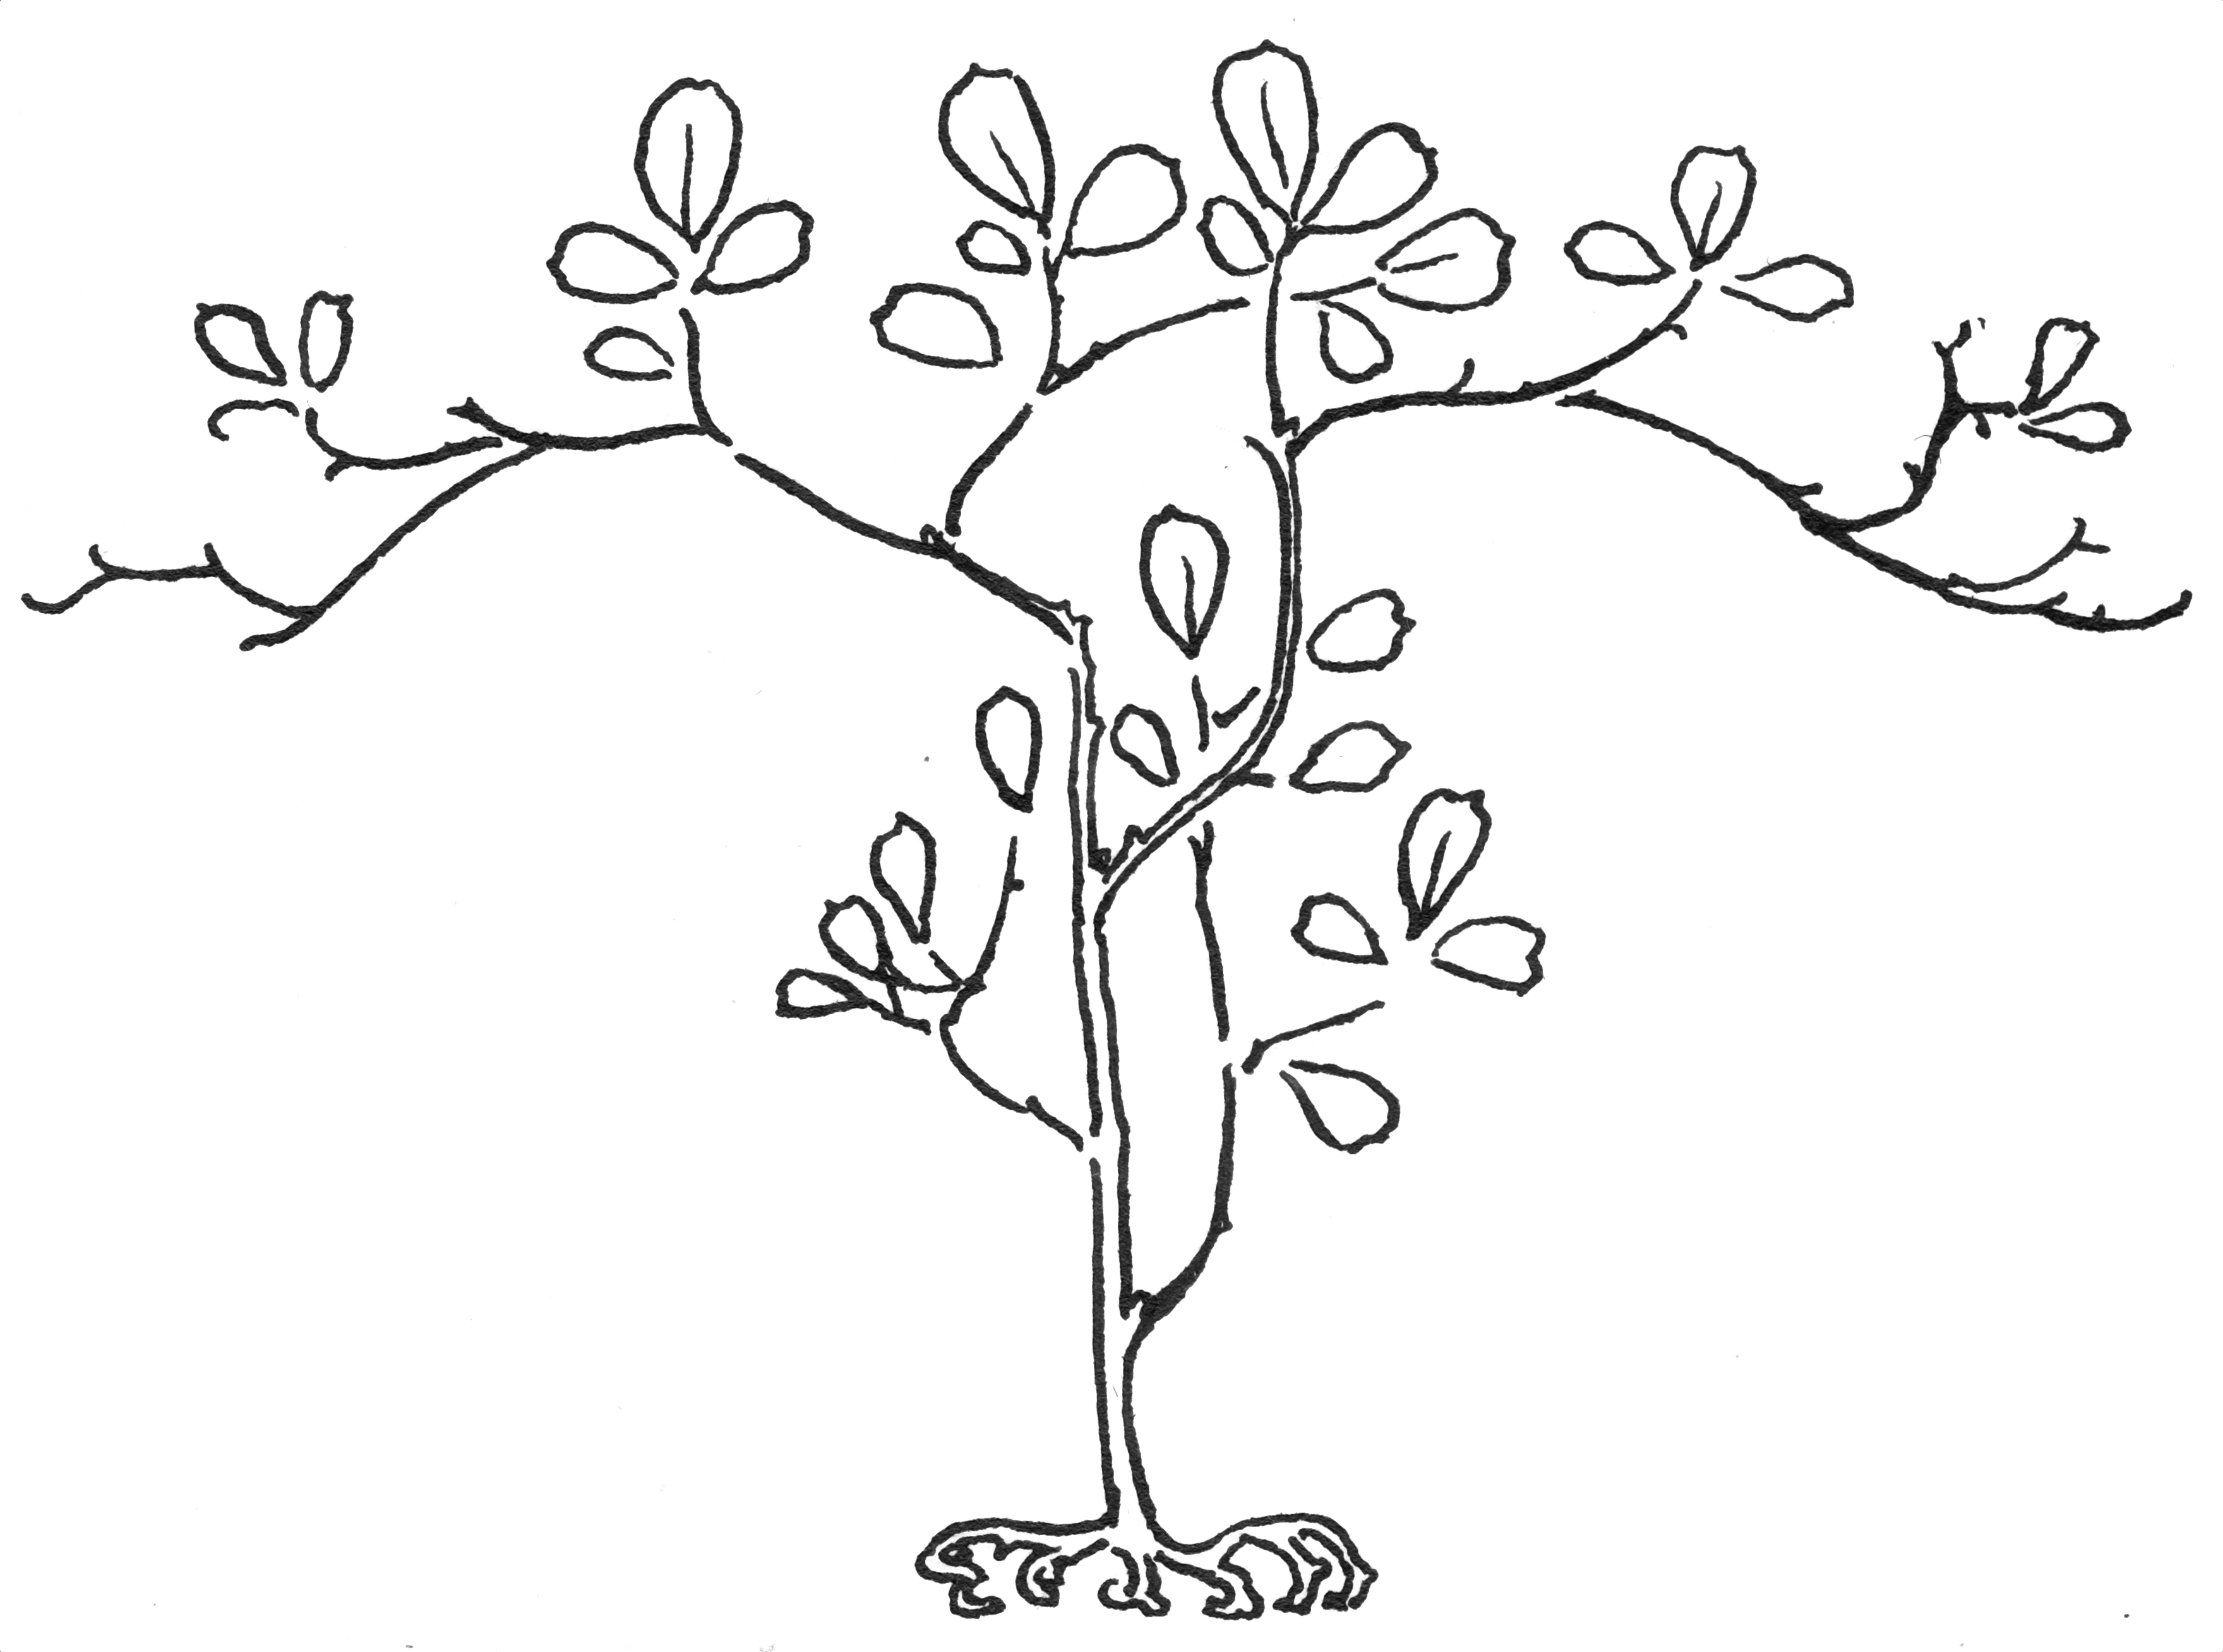
\includegraphics[width=.6\textwidth]{tree}
\end{figure}
\end{a4}